\bivtask{Modellierung mit Povray I}{5}
%
Im Verzeichnis \bivfolder{/home/bildgen/Aufgaben/povray-1} finden Sie die 
Datei \texttt{modellierung.pov}. Erweitern 
Sie dieses Povray-Skript an den markierten Stellen, damit Sie etwa 
folgendes Bild erhalten:
\begin{center}
  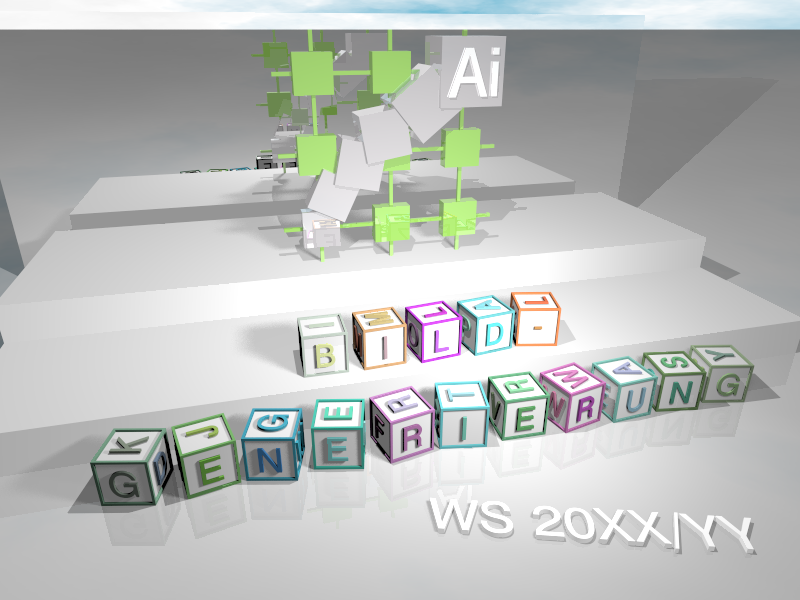
\includegraphics[width=0.75\textwidth]{modellierung.png}
\end{center}
Sie müssen
\begin{itemize}
  \item Lichtquellen,
  \item das grüne Gitter des Logos der Arbeitsgruppe „Angewandte Informatik“,
  \item die fehlenden Würfel des Textes „Bildgenerierung“,
  \item einen Teil des Podestes und
  \item den Schriftzug „WS 2021/22“
\end{itemize}
ergänzen. 
